\documentclass[a4paper,ngerman]{scrartcl}

\usepackage[utf8]{inputenc}
\usepackage{amssymb}

\usepackage[ngerman]{babel}
\usepackage{pdfpages}

\usepackage{graphicx}

\usepackage[protrusion=true,expansion=true]{microtype}

\usepackage{hyperref}
\usepackage{lmodern}
\usepackage{tabto}

\setlength\parskip{\medskipamount}
\setlength\parindent{0pt}

\usepackage{geometry}
\geometry{tmargin=1.5cm,bmargin=2cm,lmargin=1.5cm,rmargin=1.5cm}

\pagestyle{empty}

\setlength{\fboxrule}{2pt}
\setlength{\fboxsep}{-3pt}

\newcommand{\drawHere}{%
  \begin{center}%
    \fbox{\parbox[c][0.9\textwidth]{0.9\textwidth}{\ }}%
  \end{center}}

\newcommand{\header}{%
  \begin{raggedleft}
  \tiny Universität Augsburg \\
  Tag der Mathematik 2013 \par
  \end{raggedleft}}

\begin{document}

\begin{center}%
  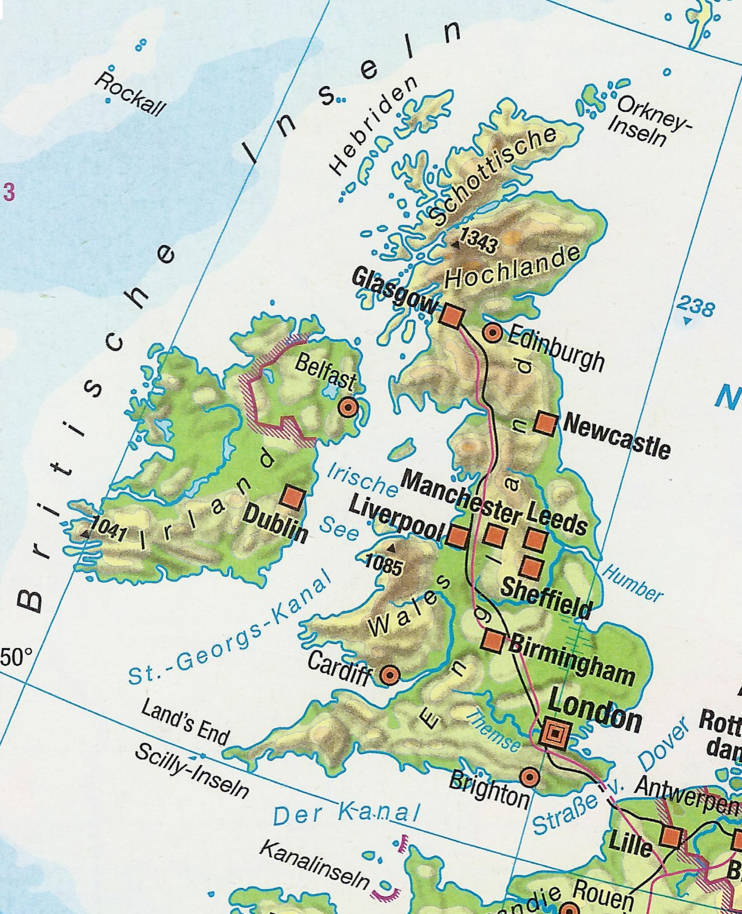
\includegraphics[scale=5]{england-grob-grob} \\
  Maßstab: $1 : 16\,000\,000$ \\
  Quelle: ...
\end{center}
\newpage

\begin{center}%
  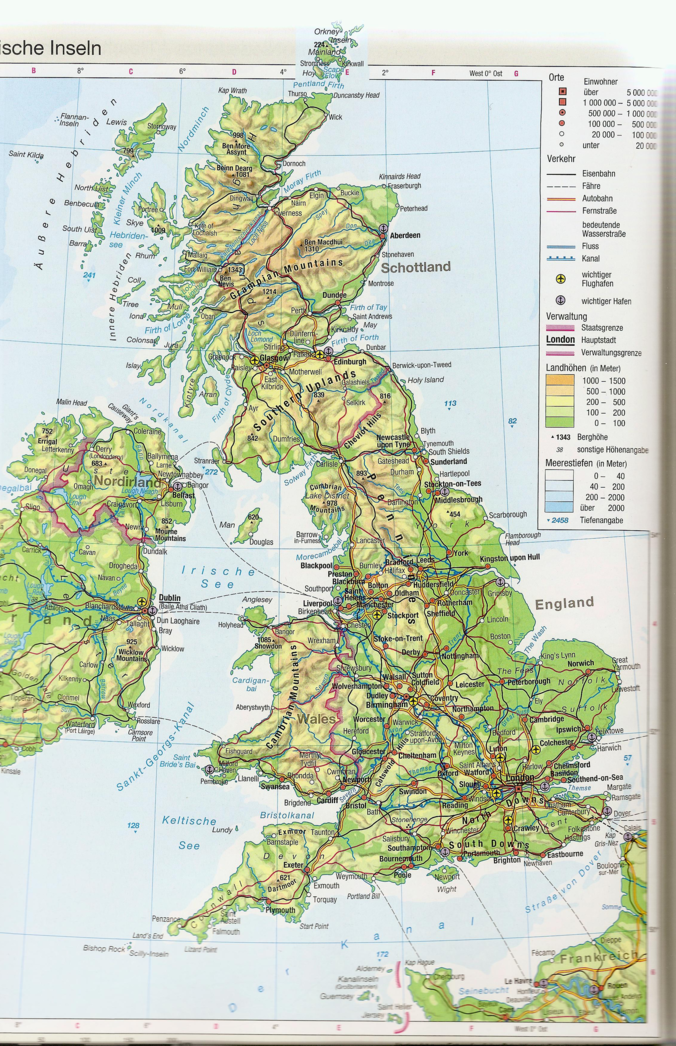
\includegraphics[scale=2.8]{england-fein-fein} \\
  Maßstab: $1 : 4\,000\,000$ \\
  Quelle: ...
\end{center}
\newpage

\header

\begin{center}
  \Huge\bf
  Die Kochsche Schneeflocke
\end{center}

\vfill
\drawHere

\vfill
\Large

\renewcommand{\labelitemi}{$\bigstar$}

\begin{itemize}
  \item So konstruiert man die Kochsche Schneeflocke:

  \begin{center}
    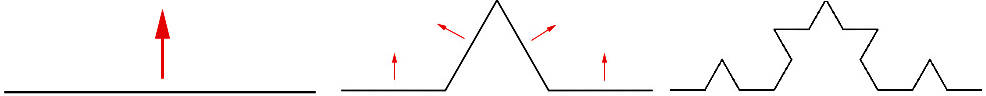
\includegraphics[scale=0.5]{koch}
  \end{center}
  \item Was ist ihr Umfang?
  \item Was ist ihr Flächeninhalt?
\end{itemize}

\newpage

\header

\begin{center}
  \Huge\bf
  Das Sierpinski-Dreieck
\end{center}

\vfill
\drawHere

\vfill
\Large

\renewcommand{\labelitemi}{$\blacktriangle$}

\begin{itemize}
  \item Spiele folgendes \emph{Chaosspiel}:
  \begin{enumerate}
    \item Zeichne ein großes gleichseitiges Dreieck.
    \item Wähle einen beliebigen Startpunkt im Dreieck.
    \item Such dir zufällig eine der drei Ecken aus.
    \item Markiere als neuen Punkt die Mitte zwischen deiner gewählten Ecke und \\ dem
    vorherigen Punkt.
    \item Fahre mit dem neuen Punkt bei Schritt 3 fort.
  \end{enumerate}
\end{itemize}

\begin{minipage}{0.9\textwidth}

\begin{itemize}
  \item Obwohl man den Startpunkt und die Ecken völlig zufällig wählt, ergibt
  sich erstaunlicherweise näherungsweise eine regelmäßige Figur: das \emph{Sierpinski-Dreieck}.
  \item Deterministisch (ohne Zufall) kann man es auch so konstruieren:

  \begin{center}
    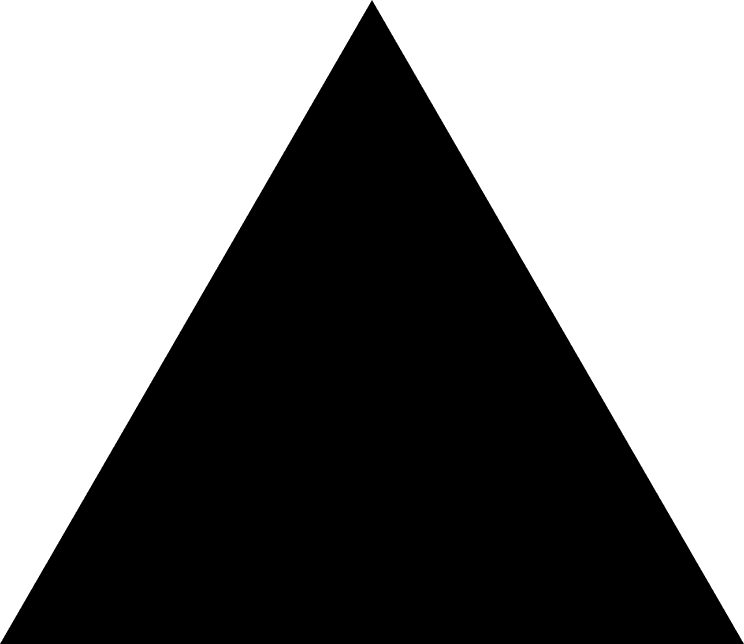
\includegraphics[scale=0.1]{sierpinski-1}\hfill
    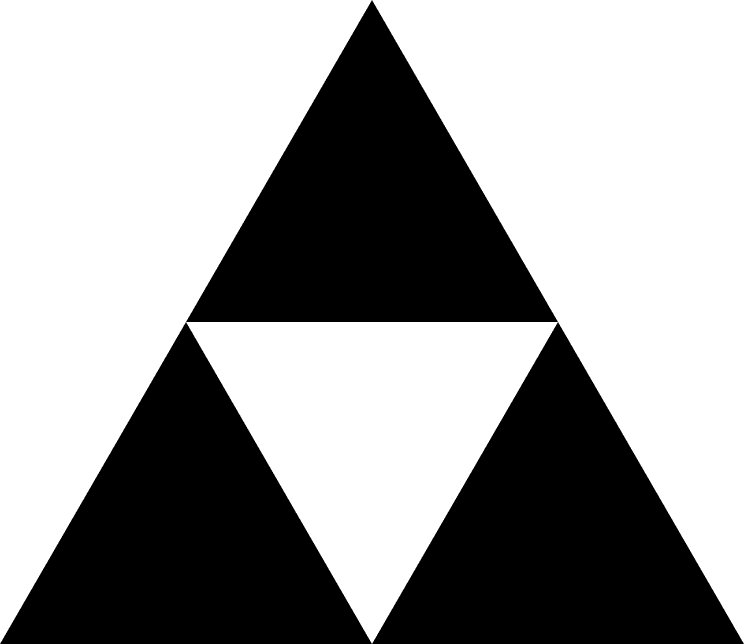
\includegraphics[scale=0.1]{sierpinski-2}\hfill
    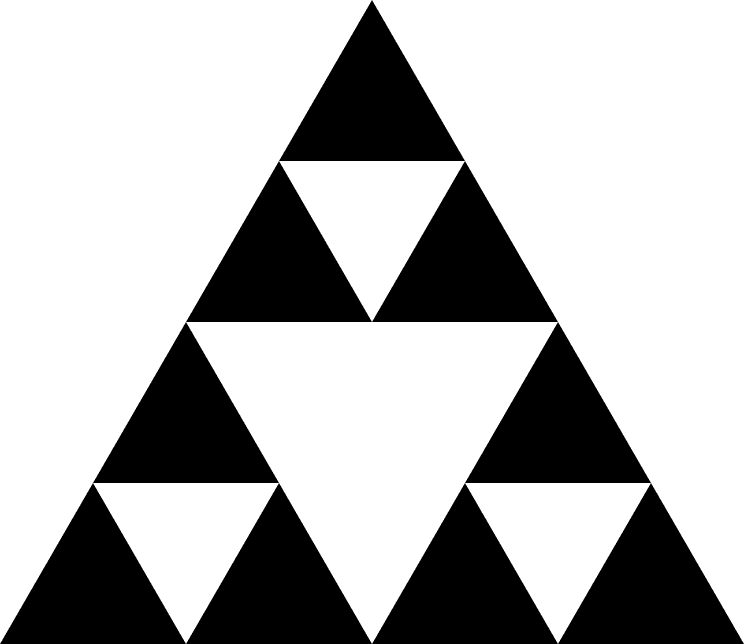
\includegraphics[scale=0.1]{sierpinski-3}\hfill
    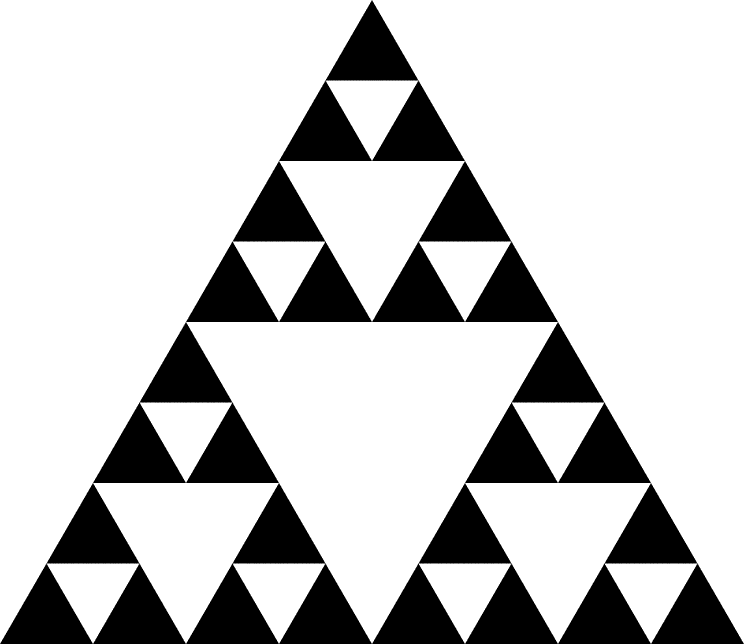
\includegraphics[scale=0.1]{sierpinski-4}
  \end{center}
  \item Wieso ergibt sich beim Chaosspiel dieses Sierpinski-Dreieck?

  Der Abstand der Punkte beim Chaosspiel zum tatsächlichen, völlig regelmäßigen
  Sierpinski-Dreieck halbiert sich mit jedem Schritt. Für das bloße Auge liegen
  daher alle Punkte (bis auf einige wenige zu Beginn) auf dem
  Sierpinski-Dreieck. Durch die zufällige Eckenwahl wird das ganze Dreieck
  gleichmäßig gefüllt.
  
  \begin{center}
    %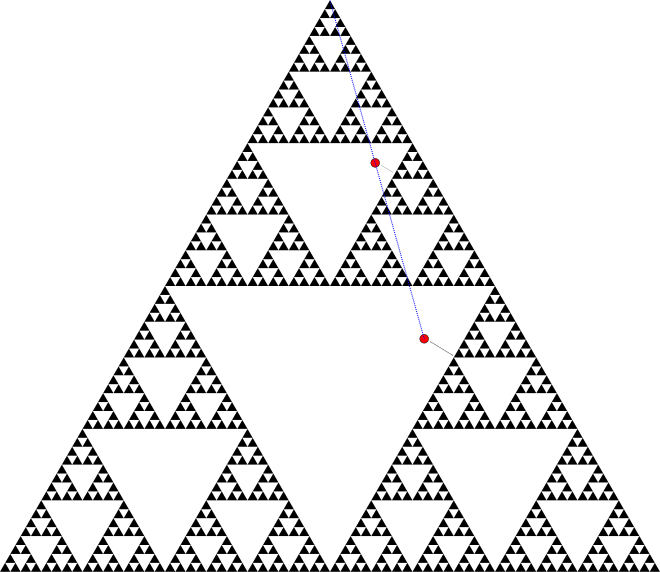
\includegraphics[scale=0.45]{sierpinski-beweis}
  \end{center}
  \item Was ist der Umfang des Sierpinski-Dreiecks?
  \item Was ist der Flächeninhalt des Sierpinski-Dreiecks?
  \item Die Kochsche Schneeflocke und das Sierpinski-Dreieck sind Beispiele für
  sog. \emph{Fraktale} (von lateinisch \emph{fractus}, "`gebrochen"').
  Annäherungen an Fraktale findet man an vielen Stellen in der Natur,
  etwa beim Romanesco-Blumenkohl, bei Flusssystemen, beim Blutkreislauf und bei
  Küstenlinien; außerdem sind manche physikalische Diagramme von fraktaler
  Natur.

  Fraktale sind
  wichtig, um sich klarzumachen, wie wunderlich geometrische Figuren sein
  können, und haben auch noch einen praktischen Nutzen: Fraktale werden
  in der Computergrafik eingesetzt, um realistisch aussehende Wälder und
  Wolken automatisiert
  generieren zu können.
\end{itemize}

\end{minipage}

\vfill
\hfill\small Chaosspiel direkt auf \url{http://xrl.us/mathechaos} spielbar

\end{document}
